\title{Gitをボトムアップから理解する}

\begin{document}

\begin{frame}
  \titlepage
\end{frame}

\begin{frame}
  \frametitle{オリジナルとライセンス}
  \begin{itemize}
  \item ``Git from the bottom up'' (Original: John Wiegley)\\
    \url{http://newartisans.com/2008/04/git-from-the-bottom-up/}
  \item ``Gitをボトムアップから理解する'' (日本語訳: O-Show)\\
    \url{http://keijinsonyaban.blogspot.jp/2011/05/git.html}
  \item ライセンス: CC-BY-SA
  \end{itemize}
\end{frame}

\begin{frame}
  \frametitle{用語集}
  リポジトリ関連
  \begin{description}
  \item[リポジトリ] コミットの集合, ワーキングツリーのアーカイブ
  \item[インデックス] 変更を登録する場所, ステージングエリア, \alert{git独自}
  \item[ワーキングツリー] リポジトリのあるディレクトリ
  \end{description}
  コミット関連
  \begin{description}
  \item[コミット] ある時点でのワーキングツリーのスナップショット
  \item[ブランチ] \alert{コミット(群)の別名}, リファレンス
  \item[タグ] \alert{コミットの別名}, 常に同じコミットを指す
  \item[master] デフォルトのことが多い\alert{単なるブランチ}
  \item[HEAD] チェックアウトされているもの
    \begin{itemize}
    \item ブランチなら、コミット操作でブランチがアップデート
    \item 特定のコミットなら、(detached HEAD), タグ名でチェックアウトしたとき等
    \end{itemize}
  \end{description}
\end{frame}

\begin{frame}
  \frametitle{基本的な概念}
  \begin{center}
    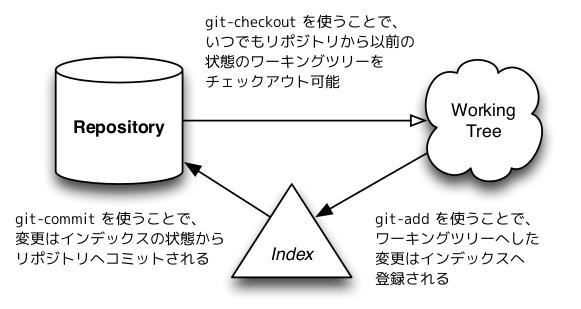
\includegraphics[height=.6\textheight]{4_ja.png}
  \end{center}
\end{frame}

\end{document}
